\documentclass{article}

\usepackage[margin=3cm]{geometry}

\usepackage{fancyhdr}
\pagestyle{fancy}
\usepackage{graphicx}
\usepackage{color}
\usepackage{xcolor}
\usepackage{hyperref}
\usepackage{cleveref}
\usepackage{tcolorbox}
%% Define no indent with line skip with new paragraph
\usepackage{parskip}

\definecolor{code}{rgb}{.92,.92,.99}
\definecolor{codered}{rgb}{.92,.62,.62}
\definecolor{darkgreen}{rgb}{.2,.62,.18}
\usepackage{listings}
\lstset{xrightmargin=10pt,xleftmargin=10pt,language=Java,captionpos=b,tabsize=3,frame=none,keywordstyle=\color{blue},commentstyle=\color{darkgreen},stringstyle=\color{red},showstringspaces=false,basicstyle=\footnotesize\ttfamily,emph={label},backgroundcolor=\color{code}}
%%numbers=left,numberstyle=\tiny,numbersep=5pt,breaklines=true,\

\usepackage{soul}
\lstdefinestyle{Bash}
{language=bash,
  escapechar=!,
  backgroundcolor=\color{white},
  columns=fullflexible,
  breaklines=true,         
  breakatwhitespace=false,
  inputencoding=utf8x,
  keywordstyle=\color{black},
  basicstyle=\small\ttfamily,
%  morekeywords={peter@kbpet},
%  alsoletter={:~$},
%  morekeywords=[2]{peter@kbpet:},
%  keywordstyle=[2]{\color{red}},
%  literate={\$}{{\textcolor{red}{\$}}}1 
%         {:}{{\textcolor{red}{:}}}1
%         {~}{{\textcolor{red}{\textasciitilde}}}1,
  literate={~}{\raisebox{-0.5ex}{\textasciitilde}}1,
}

\newenvironment{code}
{\begin{minipage}[l]{\textwidth}}
{\end{minipage}}

\newtcolorbox{mybox}{colback=blue!5!white,colframe=blue!75!black}

%\newcommand{\ccpmaketitle}[4][Roland Meertens, Christophe de Wagter, Guido de Croon, Tom van Dijk] {
%	\author{#1}
%	\title{\bf Crash Course Paparazzi 2020\\#2\\{\large #4#3}}
%	\date{February 2020}
%	\setlength{\parindent}{0em}
%	\maketitle
%}
\def\coursebranch{mavlabCourse\the\year}

% Set headers and footers
\fancyhead[LO,LE]{Crash Course Paparazzi \the\year}
\renewcommand{\chaptermark}[1]{\markboth{\chaptername\ \thechapter.\ #1}{}}
\fancyfoot[LO,LE]{{\small Crash Course Paparazzi \the\year}}
\fancyfoot[CO,CE]{\thepage}


\begin{document}
\ccpmaketitle[Tom van Dijk]{Developing your own module}{}{Part 5}

This final part is set up a bit differently than the previous ones: instead of telling you step-by-step what to do, this document will give you an overview of the concepts involved in writing your own module using the colored object detector and orange avoider as examples. You do not need to read this entire document (although you are recommended to do so), use the table of contents below to quickly find the information you need.

The simplest way to start writing your own code is by modifying the example modules: the colored object detector and orange avoider. The rest of this document will often refer to these modules as examples and describe \emph{why} they are written the way they are. Once you understand how these example modules work, you can create new or additional modules if you need them.

\tableofcontents

%\section{Conf files, airframes and modules}
%Paparazzi hierarchy:
%
%\begin{lstlisting}[language=xml]
%<conf>
%	<aircraft
%		name="bebop_orange_avoid"
%		ac_id="42"
%		airframe="airframes/tudelft/bebop_course2019_orangeavoid.xml"
%		flight_plan="flight_plans/tudelft/course2019_orangeavoid_cyberzoo.xml"
%		...
%	/>
%	...
%</conf>
%\end{lstlisting}
%
%Conf file. List of aircraft. Selected using the start.py script during Paparazzi installation. Course supplies two aircraft: orange\_avoider and orange\_avoider\_guided. You can add a new aircraft by clicking `A/C $\rightarrow$ New' in the menu bar of the Paparazzi center, or modify one of the existing course aircraft.
%
%The real magic happens inside the \emph{airframe} file.
%Airframe file: `contents' of an aircraft. Contains a list of `modules' that form the drone's behavior (e.g. state estimators, control loops, computer vision code) and tuning parameters (PID gains, color filter thresholds).
%
%\texttt{conf/airframes/tudelft/bebop\_course2019\_orangeavoid.xml}:
%\begin{lstlisting}[language=xml]
%<airframe name="bebop_avoider">
%	<description>...</description>
%	<firmware name="rotorcraft">
%		<target name="ap" board="bebop">
%			<define name="DEFINE_FOR_DRONE" value="..."/>
%			...
%		</target>
%		<target name="nps" board="pc">
%			<module name="fdm" type="gazebo"/>
%			<define name="DEFINE_FOR_SIMULATOR" value="..."/>
%			...
%		</target>
%
%		<define name="DEFINE_FOR_ALL_TARGETS" value="..."/>
%		...
%
%		<module name="MODULE"/>
%		...
%	</firmware>
%
%	<section name="...">...</section>
%	...
%</airframe>
%\end{lstlisting}
%
%
%Firmware element: defines all code that will be compiled for this airframe, by including a list of modules.
%
%Module element: placed inside firmware or inside target element. Specifies which code to be included in autopilot. Refers to a module xml file in \texttt{conf/modules} (without the .xml extension) (see \autoref{sec:files}). Most module xml files contain a description at the top of the file, followed by a list of defines that you can add to your airframe.
%
%Module: piece of behavior/code that can be added to an airframe.
%
%Flight plan: also part of an aircraft. Not discussed here, see wiki.


\section{Module code overview}
The example aircraft use the cv\_colorfilter and orange\_avoider modules to avoid obstacles.
In this part, we will take a closer look at how these modules are written and use this as an example for your own module.

\subsection{Module files}\label{sec:files}
Modules consist of the following files: a module .xml file, source and header files.  The .xml file contains a description of the module that tells Paparazzi which files to include during compilation. These xml files can be found in \texttt{paparazzi/conf/modules/}. Take for instance the orange\_avoider.xml:
\begin{lstlisting}[language=xml]
<module name="orange_avoider">
  <doc>
    ...
  </doc>
  <depends>...</depends>
  <header>
    <file name="orange_avoider.h"/>
  </header>
  <init fun="orange_avoider_init()"/>
  <periodic fun="orange_avoider_periodic()" freq="4"/>
  <makefile >
    <file name="orange_avoider.c"/>
  </makefile>
</module>
\end{lstlisting}
The xml file starts with a `module' element that sets the name of the module (orange\_avoider). Optionally, this element can contain a `dir' attribute as well, to specify the location of the source files relative to \texttt{sw/airborne/modules/}. In this case the directory is not provided and the module name is used (i.e. \texttt{sw/airborne/modules/orange\_avoider/}).

After a documentation and dependency section, the xml contains a `header' element in which the header files of the module are listed. Typically, you will only see one header file here that provides an easy-to-use access point for other modules.

The header element is followed by an `init' and `periodic' element. These specify what functions in your module code should be called by the autopilot, and in case of the periodic function it also specifies its frequency in Hz. Section \ref{sec:callbacks} will describe these functions in more detail.

At the end of the xml file is the `makefile' element. This section describes how your source files should be compiled. Simple modules such as the orange avoider only list one or more source files. More complicated modules such as \texttt{cv\_opencvdemo} can specify additional compiler flags (to link OpenCV, for example) and can have different makefile sections depending on whether the autopilot is compiled for use on the drone (\texttt{target="ap"}) or in simulation (\texttt{target="nps"}).

More information on module .xml files can be found \href{https://wiki.paparazziuav.org/wiki/Modules}{here}.

The source and header files of your module can be found in \texttt{sw/airborne/modules/<your module dir>/}. In the next sections we take a closer look at the content of these files.

When creating your own module, you can use the \texttt{create\_module} script in the \texttt{paparazzi} folder to create stubs for your module xml and the source and header files.



\subsection{Module functions}\label{sec:callbacks}
The \texttt{orange\_avoider.c} file has roughly the following structure:
\begin{lstlisting}[language=c]
#include ...

#define ...

void orange_avoider_init() {
	...
}

void orange_avoider_periodic() {
	...
}

...
\end{lstlisting}

Note that the module does not have a `main' function. This is because the module is not a stand-alone program. Instead, the autopilot will regularly call other functions that are part of your module, such as the \texttt{orange\_avoider\_init} and \texttt{orange\_avoider\_periodic} functions in this example. Which functions are called is defined by the module xml file described earlier.

The \href{https://wiki.paparazziuav.org/wiki/Modules}{Paparazzi wiki} lists the types of functions you can register in the module xml: \texttt{init}, \texttt{periodic}, \texttt{event} and \texttt{datalink}, of which init and periodic are the most relevant for this course.

The \emph{init} function is called once at startup. You can use this function to initialize important variables of your module, or for instance to subscribe to new video frames (section \ref{sec:video}).

Once the autopilot is fully initialized, it will enter an infinite loop\footnote{\texttt{sw/airborne/firmwares/rotorcraft/main.c} line 68.} in which it will continuously read new sensor data, feed this to the guidance and stabilization controllers and send new commands to the Bebop's motors\footnote{\texttt{sw/airborne/firmwares/rotorcraft/main\_ap.c handle\_periodic\_tasks} (line 202).}.
From this loop, the autopilot can also call your module's \emph{periodic} function at a frequency specified in the module xml. Within this function, you can for instance get the drone's state and use this to calculate new setpoints for the guidance controller. In the \texttt{orange\_avoider\_periodic} example, the module reads the amount of orange in the front camera image and uses this to set its next waypoint positions.

Because the periodic function is called from within the autopilot's control loop, you should take care that the function does not take too much time to run. The autopilot runs at 512~Hz, which means that it has slightly less than 2~ms to run your module code, the code of the other modules and the control loops and estimators. If your periodic function takes too long, the autopilot will run at a lower frequency than intended, which can lead to instability. In practice you have to make things pretty bad before this becomes a problem, but you should be careful when using large or nested loops in your periodic function, and video processing is best performed in the video callback function (section \ref{sec:video}) as this callback runs in a separate thread.

Together with the periodic function, the module xml can specify a \emph{start} and \emph{stop} function. These are called when the module is started or stopped, respectively. The \texttt{autorun} attribute in the module xml's \texttt{periodic} element controls whether your module is started automatically or manually; you can manually start and stop modules from the GCS by going to `Settings $\rightarrow$ System $\rightarrow$ Modules', selecting START or STOP and clicking the green checkmark.
You can find an example of start and stop functions functions in \texttt{sw/airborne/modules/loggers/file\_logger.c}, where they are used to open and close the log file.



\subsection{Handling video}\label{sec:video}
Video handling in Paparazzi works similar to the module functions described above: the autopilot will call a function in your module when a new video frame becomes available. Consider the following extract from the colorfilter module, \texttt{sw/airborne/modules/computer\_vision/colorfilter.c}:
\begin{lstlisting}[language=c]
#include "modules/computer_vision/colorfilter.h" // Includes computer_vision/cv.h!

...

struct image_t *colorfilter_func(struct image_t *img) {
	...
	return img; // Return modified image for further processing
}

void colorfilter_init(void) {
	listener = cv_add_to_device(&COLORFILTER_CAMERA, colorfilter_func, COLORFILTER_FPS);
}
\end{lstlisting}
This code fragment contains two functions: a video callback function \texttt{colorfilter\_func} and an init function \texttt{colorfilter\_init}.
As in the previous section, the init function is specified by the module xml, but this is not possible for video callbacks.
Instead, the init function uses \texttt{cv\_add\_to\_device} (from \texttt{modules/computer\_vision/cv.h}) to register the video callback function. The \texttt{cv\_add\_to\_device} function requires a video device pointer (here \texttt{\&COLORFILTER\_CAMERA}, which is set to \texttt{front\_camera} in the airframe file), the name of the callback function (\texttt{colorfilter\_func}) and the FPS at which the function should be called (\texttt{COLORFILTER\_FPS}).

After registering, the video callback is called when new frames become available.
The video callback function takes one argument: a \texttt{struct image\_t} pointer to the current camera frame. You can perform further processing of this image inside your video callback function.
At the end of the function you need to return a \texttt{struct image\_t} pointer. This pointer is then used as input for the next module that subscribed to this camera. Typically this pointer is the same as the input pointer.

The video callback function takes a pointer to the latest camera frame as argument.
This camera frame is an \texttt{image\_t} struct, as defined in \texttt{sw/airborne/modules/computer\_vision/lib/vision/image.h} (line 43).
This struct gives you access to the raw pixel values in the \texttt{buf} field.
Images in Paparazzi use a \href{https://en.wikipedia.org/wiki/YUV}{YUV color space}, where Y is the luminance (`brightness') of a pixel and U and V specify the color. Pixel colors are stored in a \href{https://www.fourcc.org/pixel-format/yuv-uyvy/}{UYVY format} which works as follows: for each pixel, two bytes of color information are used: one byte for either the U or V value, then one byte for the Y value. In other words, each pixel is described by either a (U, Y) or (V, Y) byte pair.
This means that \emph{you cannot get both the U and V value for a single pixel}! Instead, you need to read the missing U or V value from a neighboring pixel, which is a reasonable approximation in most natural images.

While it is possible to work directly with the UYVY values (as, for instance, in \texttt{image.c}'s \texttt{image\_yuv422\_colorfilt} (line 154)), it is probably easier to transform this image to an OpenCV \texttt{Mat} which allows you to use OpenCV to further process the image. An example of this can be found in \\ \texttt{sw/airborne/modules/computer\_vision/opencv\_example.cpp}:

\begin{lstlisting}[language=c++]
#include "opencv_image_functions.h"
#include <opencv2/...>
using namespace cv;

int opencv_example(char *img, int width, int height) {
	// Transform image buffer img into an OpenCV YUV422 Mat
	Mat M(height, width, CV_8UC2, img);
	// Convert to OpenCV BGR
	Mat image;
	cvtColor(M, image, CV_YUV2BGR_Y422);

	/* Do OpenCV stuff here */
	...

	// Convert back to YUV422, and put it in place of the original image
	colorrgb_opencv_to_yuv422(image, img, width, height);
	return 0;
}
\end{lstlisting}
The function first creates a \texttt{Mat} object from the image buffer, then uses OpenCV's \texttt{cvtColor} to convert it from Paparazzi's UYVY format to OpenCV's BGR. The image can then be processed as normally by OpenCV.
At the end of the function, the image is transformed back to Paparazzi's UYVY format using \texttt{colorrgb\_opencv\_to\_yuv422}. Of course, this step is only necessary if you want to pass a modified image to the next module that subscribed to this camera.

\subsubsection{Thread safety}
Unlike the module's periodic function, the video callback functions run in a separate thread from the autopilot. This means that the video callback runs \emph{in parallel} to the autopilot loop, and as a result the processing time in your callback function can exceed 2~ms without slowing down the rest of the autopilot.

Threading, however, makes it tricky to send information from the video callback to the module's periodic function, as both functions could be running in parallel and reading/writing the same variable at the same time. Threading problems are notoriously hard to debug as they often depend on the relative timing between threads, which is more-or-less random.
To prevent threading issues, variables accessed by the video thread should be protected by a \href{https://www.geeksforgeeks.org/mutex-lock-for-linux-thread-synchronization/}{\emph{mutex}}. Before accessing shared variables, a thread will attempt to lock this mutex. A mutex can only be locked once, other threads that try to lock the same mutex will wait until the mutex is unlocked again. Proper use of a mutex ensures that shared variables are accessed by only one thread at a time.
A full-on introduction of mutexes is far beyond the scope of this course, instead you are recommended to follow the example from \texttt{sw/airborne/modules/computer\_vision/cv\_detect\_color\_object.c}:
\begin{lstlisting}[language=c]
#include "pthread.h"

static pthread_mutex_t mutex;
struct color_object_t global_filter; // Variable shared by video and ap thread
                                     // Note: in the real code this is an array,
                                     // here just a variable to simplify this example.

...

// Video callback, executed in video thread
static struct image_t *object_detector(...) {
	/* Calculate object detection results */
	...

	pthread_mutex_lock(&mutex);
	global_filter = ... // Store results in global_filter
	pthread_mutex_unlock(&mutex);
	...
}

...

// Module init function
void color_object_detector_init(void) {
	...
	pthread_mutex_init(&mutex, NULL);
	...
}

// Module periodic function
// Executed in autopilot thread
void color_object_detector_periodic(void) {
	static struct color_object_t local_filter;
	pthread_mutex_lock(&mutex);
	local_filter = global_filter; // Copy results from global_filter for processing
	pthread_mutex_unlock(&mutex);
	
	/* Do stuff with local_filter */
	...
}
\end{lstlisting}
The example works as follows: this module is accessed by two threads that need to communicate with each other: a video thread that calls \texttt{object\_detector} to perform computationally intensive calculations whenever a new video frame is available, and the main autopilot thread that periodically calls \texttt{color\_object\_detector\_periodic} to further process the results of \texttt{object\_detector}.

The threads communicate through the \texttt{global\_filter} struct, which holds the object detection results that should be processed in the periodic function. Access to this struct is protected by the \texttt{mutex} object. The mutex object is initialized in the module's init function using \texttt{pthread\_mutex\_init(...)}.

When a new video frame arrives, this is processed in \texttt{object\_detector}. After processing, it will store the results in \texttt{global\_filter}. To prevent threading problems, the function will first lock the mutex using \texttt{pthread\_mutex\_lock} before it writes to \texttt{global\_filter}. After writing, it immediately releases the mutex using \texttt{pthread\_mutex\_unlock}.

A similar mechanism is used in \texttt{color\_object\_detector\_periodic} to read the \texttt{global\_filter} struct: the function first locks the mutex, then copies global\_filter to a local variable and immediately releases the lock.
Note that the periodic function does not operate directly on the \texttt{global\_filter} variable. The reason for this is that the video thread will hang as long as the periodic function has locked the mutex. After copying the results to a local variable, the \texttt{global\_filter} is no longer necessary and can be overwritten again, which means that the mutex can be unlocked \emph{before} further processing occurs and therefore the video thread does not need to wait as long.

In summary:
\begin{enumerate}
\item The video callback operates on a different thread than the rest of the autopilot. Variables that are shared between video callbacks and the rest of the code should be protected by a mutex.
\item Add a \texttt{pthread\_mutex\_t} object to your module and initialize this in your module's init function using \texttt{pthread\_mutex\_init}.
\item Before reading/writing a shared variable, lock the mutex using \texttt{pthread\_mutex\_lock}.
\item As soon as possible, release the mutex using \texttt{pthread\_mutex\_unlock}. Make a local copy of the shared variable(s) if you need more time to process them.
\end{enumerate}




\subsection{ABI: publish/subscribe messaging between modules}\label{sec:abi}
The simplest way to communicate \emph{between different modules} is to share global variables between them.
In more complex cases, however, the \href{http://wiki.paparazziuav.org/wiki/ABI}{ABI messaging system} provides an alternative to global variables.
The ABI system allows modules to publish or subscribe to messages. Compared to global variables, this has the advantage that the modules do not need to know about each other -- only about the message type -- which simplifies code maintenance and makes it easier to swap out different modules, for instance different IMU or sonar drivers.

An example of ABI messaging can be found in the colored object detector \\ (\texttt{sw/airborne/modules/computer\_vision/cv\_detect\_color\_object.c}) and the orange avoider \\ (\texttt{sw/airborne/modules/orange\_avoider/orange\_avoider.c}). In this example, the colored object detector acts as publisher and the orange avoider as subscriber. The ABI message used in this example (\texttt{VISUAL\_DETECTION}) is defined in \texttt{conf/abi.xml}, the sender ID (\texttt{COLOR\_OBJECT\_DETECTION1\_ID}) in \texttt{sw/airborne/subsystems/abi\_sender\_ids.h}:

\texttt{conf/abi.xml}:
\begin{lstlisting}[language=xml]
<protocol>
  <msg_class name="airborne">
    ...
    <message name="VISUAL_DETECTION" id="27">
      <field name="pixel_x"      type="int16_t">Center pixel X</field>
      <field name="pixel_y"      type="int16_t">Center pixel Y</field>
      <field name="pixel_width"  type="int16_t">Width in pixels</field>
      <field name="pixel_height" type="int16_t">Height in pixels</field>
      <field name="quality"      type="int32_t">Detection quality</field>
      <field name="extra"        type="int16_t">Extra field for options ...</field>
    </message>
    ...
  </msg_class>
</protocol>
\end{lstlisting}

\texttt{sw/airborne/subsystems/abi\_sender\_ids.h}:
\begin{lstlisting}[language=c]
...

/*
 * VISUAL_DETECTION communication (message 27)
*/
#ifndef COLOR_OBJECT_DETECTION1_ID
#define COLOR_OBJECT_DETECTION1_ID 1
#endif

#ifndef COLOR_OBJECT_DETECTION2_ID
#define COLOR_OBJECT_DETECTION2_ID 2
#endif

...
\end{lstlisting}

\texttt{sw/airborne/modules/computer\_vision/cv\_detect\_color\_object.c}:
\begin{lstlisting}[language=c]
#include "subsystems/abi.h"

...

void color_object_detector_periodic(void) {
	...
	AbiSendMsgVISUAL_DETECTION(COLOR_OBJECT_DETECTION1_ID,
			local_filters[0].x_c, local_filters[0].y_c,
			0, 0, local_filters[0].color_count, 0);
	...
}
\end{lstlisting}

\texttt{sw/airborne/modules/orange\_avoider/orange\_avoider.c}
\begin{lstlisting}[language=c]
#include "subsystems/abi.h"

...

#ifndef ORANGE_AVOIDER_VISUAL_DETECTION_ID
#define ORANGE_AVOIDER_VISUAL_DETECTION_ID ABI_BROADCAST
#endif
static abi_event color_detection_ev;
static void color_detection_cb(uint8_t sender_id, ...) { ... }

void orange_avoider_init(void) {
	...
	AbiBindMsgVISUAL_DETECTION(ORANGE_AVOIDER_VISUAL_DETECTION_ID,
			&color_detection_ev, color_detection_cb);
}
\end{lstlisting}

To set up communication over ABI, you should first define your message in \texttt{conf/abi.xml}. Look at the existing messages to see how you should formulate your own, then make sure you set the \texttt{id} to a value that is not in use yet. After changing the xml file, you need to run \fbox{make clean} and \fbox{make} in the paparazzi folder to generate the corresponding .c and .h files.
You should also modify \texttt{sw/airborne/subsystems/abi\_sender\_ids.h} to add one or more sender ID numbers, these are used to identify the source of the messages. Sender ID's should be unique within a message type.

Publishing messages is pretty straightforward: include the \texttt{subsystems/abi.h} header, then use \\ \texttt{AbiSendMsg<YOUR\_MESSAGE>(sender\_id, ...)} to publish a message. The first argument of this function is the sender ID, the other arguments are the fields of your message as defined in \texttt{conf/abi.xml}.

Subscribing to messages is similar to subscribing to video frames. Include the \texttt{subsystems/abi.h} header to get access to the subscribe functions. Then, use \texttt{AbiBindMsg<YOUR\_MESSAGE>(sender\_id, ev, cb)} to subscribe to this message class.
AbiBindMsg takes the following arguments: a \texttt{sender\_id}, which is used to filter messages by their source ID. Set this sender\_id to \texttt{ABI\_BROADCAST} to accept messages from all senders. The second argument is a pointer to an \texttt{abi\_event} that you declare somewhere in your code (here \texttt{color\_detection\_ev}). Finally, the third argument is a pointer to your callback function which gets called whenever a new message is published. The callback function takes as arguments the \texttt{sender\_id}, followed by the fields defined for this message class.

ABI callbacks run in the thread that called \texttt{AbiSendMsg}, which in practice should be the autopilot thread (do \emph{not} call AbiSendMsg from the video thread!). This means that you do not need to use mutexes to get/set global variables from the callback, but also that you should take care that your callback does not take too much time.




\subsection{Getting the drone's state}
At some point in your module, you may want to get the current state of the drone.
An example can be found in \texttt{sw/airborne/modules/orange\_avoider/orange\_avoider.c}, where the drone's position and heading are used to update the location of the next waypoint:
\begin{lstlisting}[language=c]
#include "state.h"

...

static uint8_t calculateForwards(struct EnuCoor_i *new_coor, float distanceMeters)
{
  float heading  = stateGetNedToBodyEulers_f()->psi;

  // Now determine where to place the waypoint you want to go to
  new_coor->x = stateGetPositionEnu_i()->x + 
      POS_BFP_OF_REAL(sinf(heading) * (distanceMeters));
  new_coor->y = stateGetPositionEnu_i()->y +
      POS_BFP_OF_REAL(cosf(heading) * (distanceMeters));
  VERBOSE_PRINT("Calculated %f m forward position. x: %f  y: %f "
                "based on pos(%f, %f) and heading(%f)\n", distanceMeters,	
                POS_FLOAT_OF_BFP(new_coor->x), POS_FLOAT_OF_BFP(new_coor->y),
                stateGetPositionEnu_f()->x, stateGetPositionEnu_f()->y,
                DegOfRad(heading));
  return false;
}

...
\end{lstlisting}
To get the drone's current state, include the \texttt{state.h} header. Then, the state can be accessed using the \texttt{stateGet...} functions. Scroll through the \texttt{state.h} header to get an idea of the values you can access.

State.h uses the following naming conventions: functions ending in \texttt{\_f} return the drone's state in a floating-point format (recommended). These are the easiest to work with, but can be more computationally intensive on small microcontrollers. Functions ending in \texttt{\_i} return the current state in a Binary Fixed-Point (BFP) format. The \texttt{\_BFP\_OF\_REAL} and \texttt{\_FLOAT\_OF\_BFP} macros in \\ \texttt{sw/airborne/math/pprz\_algebra\_int.h} allow you to convert data between these formats.

The drone's state can be expressed in different coordinate frames. For this course, the North-East-Down (\texttt{Ned}) and East-North-Up (\texttt{Enu}) frames are likely the most relevant. Positions in these frames are expressed relative to the flight plan origin, which for the example flight plans lies in the center of the Cyberzoo. Angular rates and Euler angles are expressed in the body frame, which follows a Front-Right-Down convention.


\subsection{Navigation and guidance commands}
To avoid obstacles, your module will at some point need to control where the drone is going. Depending on the level of control you want there are multiple ways to achieve this.

\subsubsection{NAV mode}
The \href{https://wiki.paparazziuav.org/wiki/Flight_Plans}{flight plan} lets you describe an entire flight or mission and lets you give high-level commands to the drone, such as waypoint sequences to follow. The flight plan by itself does not give you fine-grained enough control to avoid obstacles, and will therefore not be discussed in further detail here.

You can, however, interact with the flight plan and waypoints from within your own module, which is the method used in \texttt{sw/airborne/modules/orange\_avoider/orange\_avoider.c}. Consider the following flight plan and code extracts:

\texttt{conf/flight\_plans/tudelft/course2019\_orangeavoid\_cyberzoo.xml}:
\begin{lstlisting}[language=xml]
<flight_plan ...>
	...
	<waypoints>
		...
		<waypoint name="GOAL" x="1.9" y="1.0"/>
		...
	</waypoints>
	...
	<blocks>
		...
		<block name="START" ...>
			<call_once fun="NavSetWaypointHere(WP_GOAL)"/>
			<stay wp="GOAL"/>
		</block>
	</blocks>
</flight_plan>
\end{lstlisting}

\texttt{sw/airborne/modules/orange\_avoider/orange\_avoider.c}:
\begin{lstlisting}[language=c]
#include "firmwares/rotorcraft/navigation.h"

...

uint8_t moveWaypointForward(uint8_t waypoint, float distanceMeters);
uint8_t moveWaypoint(uint8_t waypoint, struct EnuCoor_i *new_coor);

...

void orange_avoider_periodic(void) {
	/* State machine logic left out for this example */
	moveWaypointForward(WP_GOAL, moveDistance);
	...
}

uint8_t moveWaypoint(uint8_t waypoint, struct EnuCoor_i *new_coor)
{
  waypoint_set_xy_i(waypoint, new_coor->x, new_coor->y);
  return false;
}

uint8_t moveWaypointForward(uint8_t waypoint, float distanceMeters)
{
  struct EnuCoor_i new_coor;
  calculateForwards(&new_coor, distanceMeters);
  moveWaypoint(waypoint, &new_coor);
  return false;
}
\end{lstlisting}

In this example, the flight plan does not seem to do much: in the \texttt{START} block, it first places the \texttt{GOAL} waypoint at the drone's current position, then stays at this waypoint. Indeed, without the orange avoider module the drone would just stay in place. The avoidance behavior in this case comes from the orange\_avoider's periodic function. In this function it moves the GOAL waypoint to a new location. Because the drone is commanded to stay at this waypoint, it will move to follow it.

Using the flight plan and waypoints works, but has its limitations. While you can control where the drone is going, it is not possible to control the drone's velocities. Furthermore, this method assumes that the drone's position is fully known, which may not always be the case such as when flying without Optitrack.

\subsubsection{GUIDED mode}
As an alternative, the drone can be controlled in GUIDED mode. In this mode, your module can directly send setpoints to the guidance controller, including setpoints for the drone's velocity. An example is provided in \texttt{sw/airborne/modules/orange\_avoider/orange\_avoider\_guided.c} and the corresponding flight plan:

\texttt{conf/flight\_plans/tudelft/course2019\_orangeavoid\_cyberzoo\_guided.xml}:
\begin{lstlisting}[language=xml]
<flight_plan ...>
	<header>
		...
		inline void setNav(void) {
			autopilot_mode_auto2 = AP_MODE_NAV;
			autopilot_static_set_mode(AP_MODE_NAV);
		}
		inline void setGuided(void) {
			autopilot_mode_auto2 = AP_MODE_GUIDED;
			autopilot_static_set_mode(AP_MODE_GUIDED);
		}
	</header>
	...
	<blocks>
		...
		<block name="START" ...>
			<call_once fun="setGuided()"/>
			<stay wp="STDBY"/>
		</block>
		<block name="STOP">
			<call_once fun="NavSetWaypointHere(WP_STDBY)"/>
			<call_once fun="setNav()"/>
			<stay wp="STBDY"/>
		</block>
		...
		<block name="Land here" ...>
			<call_once fun="setNav()"/>
			...
		</block>
	</blocks>
</flight_plan>
\end{lstlisting}

\texttt{sw/airborne/modules/orange\_avoider/orange\_avoider\_guided.c}:
\begin{lstlisting}[language=c]
#include "firmwares/rotorcraft/guidance/guidance_h.h"

...

void orange_avoider_guided_periodic(void) {
	if (guidance_h.mode != GUIDANCE_H_MODE_GUIDED) {
		return;
	}

	/* State machine logic left out for this example */
	guidance_h_set_guided_body_vel(speed_sp, 0);
	...
}
\end{lstlisting}

In this example, the module uses \texttt{guidance\_h\_set\_guided\_body\_vel} to send a velocity setpoint to the guidance controller. However, when the drone is in NAV mode, it will ignore these commands and follow the navigation commands from the flight plan instead.

To switch the autopilot to GUIDED mode, two extra functions were added in the flight plan header: \texttt{setNav} and \texttt{setGuided}. Calling these functions sets the autopilot mode to NAV or GUIDED, respectively. This is exactly what happens in the \texttt{START} block: the drone is commanded to stay at the STDBY waypoint, but just before that the autopilot is switched to GUIDED mode by calling \texttt{setGuided}. As a result, the drone will ignore the stay command and follow the module's setpoints instead. In the \texttt{STOP} block, the autopilot is switched back to NAV mode and stays at the STDBY waypoint.

You should take special care that the drone is in the correct mode at the start of each block. For instance, forgetting to switch the drone back from GUIDED mode to NAV in the \texttt{Land here} block would cause it to ignore the landing command, even when the landing was triggered by a safety exception! It is therefore best practice to call the \texttt{setNav} or \texttt{setGuided} function at the start of each block to ensure that the autopilot is in the correct mode.

\subsubsection{MODULE mode}
For completeness, it should be mentioned that your module can also \emph{replace} the entire guidance or even stabilization controller. This can be achieved by switching the autopilot to MODULE mode. In module mode, the autopilot will call the \texttt{guidance\_h\_module\_run} and \texttt{guidance\_v\_module\_run} functions during its main loop, your module should provide these functions.

Two examples of MODULE mode controllers are provided in \texttt{sw/airborne/modules/ctrl/ctrl\_module\_innerloop\_demo.c} and \texttt{\_outerloop\_demo.c}. In MODULE mode \emph{you} are responsible for the drone's stability, therefore we recommend you to stick to NAV or GUIDED mode during the course.




\subsection{Defines and settings}\label{sec:settings}
Your module will most likely contain tunable parameters, such as the minimum and maximum YUV values for which a pixel is considered an obstacle. While you can write these numbers directly in your code, this will make it difficult to tune them later. Paparazzi provides two systems to simplify parameter tuning: defines and settings.

Defines allow you to set constant values from the airframe file. See, for example, the following abstract of the \texttt{bebop\_course2019\_orangeavoid.xml} airframe:
\begin{lstlisting}[language=xml]
<airframe ...>
	<firmware ...>
		<target name="ap" board="bebop">
			<define name="COLOR_OBJECT_DETECTOR_LUM_MIN1" value="40"/>
			...
		</target>
		...
		<define name="ARRIVED_AT_WAYPOINT" value="0.5"/>
		...
		<module name="cv_detect_color_object">
			<define name="COLOR_OBJECT_DETECTOR_CAMERA1" value="front_camera"/>
			...
		</module>
	</firmware>
	...
	<section name="GUIDANCE_H" prefix="GUIDANCE_H_">
		<define name="CLIMB_VSPEED" value="1.0"/>
	</section>
	...
</airframe>
\end{lstlisting}

As you can see, defines can be set at multiple places in the airframe file. The behavior is mostly the same in these cases, with the following exceptions:
\begin{itemize}
\item Defines placed in the \texttt{<target>} elements are only set when the autopilot is built for that target, i.e. \texttt{"ap"} for the real drone and \texttt{"nps"} for the simulator. This allows you to, for instance, use different color filter settings on the real and simulated drone.
\item Placing a define inside a \texttt{<module>} element has no special effect! The define is also visible in other modules, so be sure to use a unique name. Typically, defines are prefixed with the name of the module (e.g. \texttt{COLOR\_OBJECT\_DETECTOR\_}) to make them unique. The only reason these defines are placed inside the module element is to improve readability.
\item \texttt{<section>} elements allow you to specify a \texttt{prefix}, this prefix is placed in front of all define names inside this section. In the example, the \texttt{CLIMB\_VSPEED} define is available in the code as \texttt{GUIDANCE\_H\_CLIMB\_VSPEED}.
\end{itemize}
During compilation, these defines are turned into preprocessor macros and can be referred to directly from your code.


Airframe defines allow you to set constant parameters at compile-time, but in some cases it would be easier if you could change these values during the flight. This is possible with the \href{https://wiki.paparazziuav.org/wiki/Settings}{`settings'} mechanism. Settings are defined in the module xml file. Take for example \texttt{conf/modules/cv\_detect\_color\_orange.xml}:
\begin{lstlisting}[language=xml]
<module name="cv_detect_color_object" ...>
	...
	<settings>
		<dl_settings name="ColorObjectDetector">
			<dl_setting var="cod_lum_min1" min="0" step="1" max="255" shortname="y_min1"/>
			...
		</dl_settings>
	</settings>
</module>
\end{lstlisting}
Settings listed in the module xml can be \href{https://wiki.paparazziuav.org/wiki/GCS#Settings}{tuned from the Ground Control Station} by going to the `Settings' tab and then selecting the tab belonging to your module, as defined in the \texttt{dl\_settings} element (here \texttt{ColorObjectDetector}). To read the current value of a parameter from the drone, click its value (the number) in the GCS. Te set a value on the drone, adjust the slider, \emph{then click the green checkmark} to upload this new value to the drone. Click the value number again to make sure the setting was updated.

Use the \texttt{dl\_setting} element in your module xml to add a setting to your module. The \texttt{var} attribute specifies the variable this setting should be written to; this variable should be globally accessible. The \texttt{min}, \texttt{step} and \texttt{max} attributes let you specify a range of possible values for this setting. Finally, using \texttt{shortname} you can control the name under which this setting is listed in the GCS.

It is possible to combine the define and settings mechanisms, where the define provides a default value that can be adjusted later using settings. This often uses the following pattern:
\begin{lstlisting}[language=c]
#ifndef MY_DEFINE
#define MY_DEFINE 0
#endif
int my_setting = MY_DEFINE;
\end{lstlisting}
In this example, \texttt{MY\_DEFINE} provides the initial value of \texttt{my\_setting}. MY\_DEFINE can be set from the airframe file, but if it is not defined there this code will give it a default value of 0. The actual parameter is stored in \texttt{my\_setting}, for which a \texttt{<dl\_setting>} element is included in the module's xml file.





\section{Logging}\label{sec:logging}
While writing your module, you will likely want feedback on what is happening in your code while the module is running. Especially when things go wrong (and they will), logging is essential in tracking down and fixing problems. In this section you will find a brief overview of approaches to logging.

\subsection{Printing to terminal}
Perhaps one of the easiest approaches to logging is to make your module print messages to a terminal. While running the simulations of the earlier parts, you may already have noticed that the example modules print information to the terminal in the Paparazzi Center:
\begin{lstlisting}
[orange_avoider->calculateForwards()] Calculated 1.000000 m forward position.
  x: -0.164062  y: 0.968750 based on pos(-0.007860, -0.017677) and heading(-9.120324)
[orange_avoider->moveWaypoint()] Moving waypoint 5 to x:-0.164062 y:0.968750
\end{lstlisting}
You can add your own debug messages as follows: first, include the \texttt{<stdio.h>} header to get access to the \texttt{printf} function. Then, at any point in your code, use \href{http://www.cplusplus.com/reference/cstdio/printf/}{\texttt{printf}} to print your debug message. Printf requires a format string to know how to print the variables you specify, follow the link to find out more.

When running in simulation the printf messages will automatically appear in the Paparazzi Center. You can also read these messages on the real drone using the following steps:
\begin{enumerate}
\item Open a terminal window (Ctrl+Alt+T)
\item Make sure you are connected to the drone's WiFi access point, the open a telnet connection using \fbox{telnet 192.168.42.1}.
\item Navigate to the Paparazzi folder using \fbox{cd data/ftp/internal\_000/paparazzi}.
\item You need to restart the autopilot for the messages to show up. Run \fbox{killall -9 ap.elf}, then \fbox{./ap.elf} to restart the autopilot.
\item When you are finished and the drone is landed, kill the autopilot by pressing Ctrl+C twice, then disconnect using Ctrl+D.
\end{enumerate}


\subsection{Telemetry}
Paparazzi also provides a \href{https://wiki.paparazziuav.org/wiki/Telemetry}{telemetry} system to track and plot variables in real-time.
Adding your own telemetry message requires you to change multiple files, which will be summarized here.

First of all you need to define your telemetry message. For this, you will need to edit \texttt{conf/messages.xml}, but if you are running a clean installation of Paparazzi this file will not exist. Copy this file from \texttt{sw/ext/pprzlink/message\_definitions/v1.0/} and paste it in the \texttt{conf/} folder. This will override the default messages provided by \href{https://github.com/paparazzi/pprzlink}{pprzlink} and allow you to add your own.
The \texttt{messages.xml} file contains a collection of message types, their id numbers and their fields. The file looks as follows:
\begin{lstlisting}[language=xml]
<protocol>
	<msg_class name="telemetry" id="1">
		...
		<message name="DRAGSPEED" id="38">
			<description>...</description>
			<field name="u_est" type="float" unit="m/s"/>
			...
		</message>
		...
	</msg_class>
</protocol>
\end{lstlisting}
The \texttt{message} element describes a message class. Each message class is given a unique \texttt{id} number between 0 and 255. Most id numbers are already taken, you can find out which ones are free by running \fbox{./sw/tools/find\_free\_msg\_id.out} from the paparazzi folder or by looking for comments such as \texttt{<!-- 45 is free -->}.
The message itself is defined by a collection of \texttt{field}s, for which you need to specify the \texttt{name}, data \texttt{type} and optionally a \texttt{unit}.

Paparazzi needs to generate c code to send and receive your message class. After changing the messages.xml file, you will need to remake Paparazzi. Close paparazzi if it is still running, open a terminal (Ctrl+Alt+T), go to the paparazzi folder \fbox{cd paparazzi} and run \fbox{make clean \&\& make}.

After adding your message class, you need to inform Paparazzi that it should actually send this message. For this you need to edit the drone's telemetry xml, which in the example aircraft is \texttt{conf/telemetry/default\_rotorcraft.xml}:
\begin{lstlisting}[language=xml]
<telemetry>
	<process name="Main">
		<mode name="default" ...>
			...
			<message name="DRAGSPEED" period="0.02"/>
		</mode>
		...
	</process>
</telemetry>
\end{lstlisting}
Now, Paparazzi will know that it has to send the message, but it does not know \emph{how} yet.

For this, you will need to edit your module. We take the dragspeed module \\ (\texttt{sw/airborne/modules/dragspeed/dragspeed.c}) as an example:
\begin{lstlisting}[language=c]
#include "subsystems/datalink/telemetry.h"

...

void dragspeed_init(void) {
	...
	// Register callbacks
	register_periodic_telemetry(DefaultPeriodic, PPRZ_MSG_ID_DRAGSPEED, send_dragspeed);
	...
}

...

static void send_dragspeed(struct transport_tx *trans, struct link_device *dev) {
	// Calculate INS velocity in body frame
	...
	// Send telemetry message
	pprz_msg_send_DRAGSPEED(trans, dev, AC_ID, &dragspeed.vel.x, &dragspeed.vel.y,
			&vel_ins_body.x, &vel_ins_body.y);
}
\end{lstlisting}
In the module's init function, it registers a callback function to send the DRAGSPEED telemetry message. The callback is registered using \texttt{register\_periodic\_telemetry}, which takes as arguments a periodic\_telemetry pointer (keep this one at \texttt{DefaultPeriodic}), the ID number of your message class (\texttt{PPRZ\_MSG\_ID\_<YOUR MESSAGE NAME>}), and the callback function.

The callback function, here \texttt{send\_dragspeed}, will actually send the telemetry message. The function takes two arguments: a \texttt{struct transport\_tx *trans} and a \texttt{struct link\_device *dev}. You do not need to use or understand these structs, you only need to pass them along to the \texttt{pprz\_msg\_send\_<YOUR MESSAGE NAME>} function. Call this function with \texttt{trans, dev, AC\_ID} as the first three arguments, the following arguments are pointers to the fields of your message.

To receive your telemetry messages, go to the Paparazzi Center, make sure your session is running, then click `Tools $\rightarrow$ Messages'. To plot your telemetry values over time, click `Tools $\rightarrow$ Real-time Plotter', then drag the telemetry message field from the `Messages' window to the `Plotter' window. Use the sliders in the plotter window to adjust the update rate and timespan of the plotter.


\subsection{Video streaming}
When developing computer vision modules, it can be helpful to view the camera images of the drone, possibly with annotations by your module. The \texttt{video\_rtp\_stream} module lets you stream video back to your pc; this module has already been added to the example airframes.

To receive the video stream, start VLC and open \texttt{sw/tools/rtpviewer/rtp5000.sdp} to view \texttt{VIEWVIDEO\_CAMERA} (the front camera) and \texttt{sw/tools/rtpviewer/rtp6000.sdp} to view \texttt{VIEWVIDEO\_CAMERA2} (the bottom camera). Note that there might be a delay on the video; this delay is caused by the video streaming and is not visible to the modules.


\subsection{CSV file logging}
Printing to terminal, telemetry and video streaming give you live feedback of your drone's behavior, but for some purposes it might be useful to analyze the results in more detail after the flight. To help you with this, we have included a CSV file logger module (\texttt{logger\_file}) that will periodically write the values of important variables to a csv file that you can analyze later using python or matlab.

The csv logger is already included in the example airframes. To start logging, go to the `Settings' tab in the GCS, then to `System $\rightarrow$ Modules'. Set \texttt{file\_logger\_periodic} to START and press the green checkmark to start recording. After your flight, press STOP, then the green checkmark to stop recording and save the csv file.

You can change the variables that are being logged by editing \texttt{sw/airborne/modules/loggers/file\_logger.c}:
\begin{lstlisting}[language=c]
...

static void file_logger_write_header(FILE *file) {
  fprintf(file, "time,");
  fprintf(file, "pos_x,pos_y,pos_z,");
  fprintf(file, "vel_x,vel_y,vel_z,");
  fprintf(file, "att_phi,att_theta,att_psi,");
  fprintf(file, "rate_p,rate_q,rate_r,");
  fprintf(file, "cmd_thrust,cmd_roll,cmd_pitch,cmd_yaw\n");
}

static void file_logger_write_row(FILE *file) {
  struct NedCoor_f *pos = stateGetPositionNed_f();
  struct NedCoor_f *vel = stateGetSpeedNed_f();
  struct FloatEulers *att = stateGetNedToBodyEulers_f();
  struct FloatRates *rates = stateGetBodyRates_f();

  fprintf(file, "%f,", get_sys_time_float());
  fprintf(file, "%f,%f,%f,", pos->x, pos->y, pos->z);
  fprintf(file, "%f,%f,%f,", vel->x, vel->y, vel->z);
  fprintf(file, "%f,%f,%f,", att->phi, att->theta, att->psi);
  fprintf(file, "%f,%f,%f,", rates->p, rates->q, rates->r);
  fprintf(file, "%d,%d,%d,%d\n",
      stabilization_cmd[COMMAND_THRUST], stabilization_cmd[COMMAND_ROLL],
      stabilization_cmd[COMMAND_PITCH], stabilization_cmd[COMMAND_YAW]);
}

...
\end{lstlisting}
The function \texttt{file\_logger\_write\_header} writes the column names in the first line of the csv file. Then, for each periodic function call, \texttt{file\_logger\_write\_row} writes a new row to the csv file. When modifying the file logger, make sure that the fprintf's in write\_row match the column names of write\_header. Also, do not forget to end the final fprintf statements with a `\textbackslash n' to end the line!

When logging from the simulator, you can find the csv files in \texttt{/tmp/paparazzi/log/<timestamp>.csv}.
Section \ref{sec:ftp} will show how to download the csv files from the real drone.


\subsection{Video capture}
To help you develop vision algorithms, the \texttt{video\_capture} module lets you record camera images from your drone (both in simulation and on the real drone). The module is already included in the example airframe files. To start and stop recording, use the buttons in the top-left of the GCS.

Video frames recorded in the simulator can be found in \texttt{/tmp/paparazzi/images/<timestamp>/}. the images are named with a timestamp in microseconds since the autopilot was started, this timestamp matches the one recorded by the csv file logger. Section \ref{sec:ftp} will show how to download the images from the real drone.

(Note: the image folder name is determined at the start of the autopilot, not the start of recording. If you record multiple videos during one flight, they will be stored in the same folder.)


\subsection{Downloading log files through FTP}\label{sec:ftp}
After recording your log and/or video files, you can download them from the real drone over FTP using the following steps:
\begin{enumerate}
\item Make sure you are connected to the drone's WiFi access point.
\item Open Ubuntu's file browser.
\item On the left, click `Connect to Server'.
\item Enter \fbox{ftp://192.168.42.1} as the server address.
\item Click `Connect As $\rightarrow$ Anonymous' then click `Connect'.
\item You can now access the drone's file system. The log files are stored in \texttt{internal\_000/log/}, the video frames in \texttt{internal\_000/images/}. Use the file browser to copy them to your pc. (Note: depending on your version of Ubuntu, you may need to use `Right click $\rightarrow$ Copy' instead of Ctrl+C to copy the files).
\end{enumerate}



\section{Testing}
During development, you will regularly want to test your code to check that everything works as expected. While it is tempting to test everything on the real drone, this is often time-consuming and risky. Instead, we recommend you to do a large part of your testing off-board. A large part of development can be done on datasets that you collected beforehand (see the previous section), and closed-loop tests can be performed in simulation before the code is finally tested on the real drone.


\subsection{Offline development with Python and OpenCV}
While it is possible to develop your vision algorithms directly in Paparazzi, the frequent recompiling and lack of interactivity of c makes this a time-consuming process.
Instead, we suggest that you prototype your vision algorithms in Python. Python code is in general a bit easier to write, but the biggest advantage of Python is that you can run it interactively (IPython). This makes it significantly easier to try out stuff and play around with the functions that OpenCV has to offer.

In this section we show how to install and use Python (3), OpenCV and Spyder. Spyder is a python editor that is aimed specifically at scientific computing and has excellent IPython support. As for the actual development of your vision code: that is something we leave up to you.

%\subsubsection{Installation}
To start the installation, use apt to install the most important components. Open a terminal (Ctrl+Alt+T) and enter:
\begin{lstlisting}[language=bash]
sudo apt install python3 pip3 virtualenv spyder3
\end{lstlisting}

Next, you need to install OpenCV for python. It is possible to do a system-wide installation of OpenCV, however the Bebop uses an older version of openCV (3.4.5) that we would like to match in python. For obvious reasons, installing an outdated version of a library on your entire system is not ideal. Instead, we will set up a virtual environment (a stand-alone version of python and its libraries) that we will install opencv to.
\begin{enumerate}
\item Open a terminal (Ctrl+Alt+T)
\item Create a new folder to store your virtual environment:
\begin{lstlisting}[language=bash]
mkdir -p ~/envs/mavlabcourse
cd ~/envs/mavlabcourse
\end{lstlisting}
\item Create the virtual environment:
\begin{lstlisting}[language=bash]
virtualenv -p python3 env
\end{lstlisting}
\end{enumerate}

Now we need to install opencv to this virtual environment. Use to following steps to install opencv (and other packages):
\begin{enumerate}\setcounter{enumi}{3}
\item Activate the virtual environment:
\begin{lstlisting}[language=bash]
source env/bin/activate
\end{lstlisting}
You should now see \texttt{(env)} before the terminal prompt.
\item Install opencv 3.4.5:
\begin{lstlisting}[language=bash]
pip3 install opencv-python==3.4.5.20
\end{lstlisting}
\item To simplify plotting and drawing, we will also install matplotlib (\href{https://matplotlib.org/api/pyplot_api.html}{pyplot}):
\begin{lstlisting}[language=bash]
pip3 install matplotlib
\end{lstlisting}
\item When you are finished installing packages, run \fbox{deactivate} to deactivate the virtual environment. The \texttt{(env)} should disappear.
\item Set up Spyder to use the virtual environment:
\begin{itemize}
\item Launch Spyder:
\begin{lstlisting}[language=bash]
spyder3
\end{lstlisting}
\item Set up the python interpreter. In the menu, click `Tools $\rightarrow$ Preferences'. Navigate to `Python interpreter'. Select `Use the following Python interpreter', then click the file button and select the \texttt{python3} executable in your environment's \texttt{bin} folder (\verb|~/envs/mavlabcourse/env/bin/python3|).
\item Click `Apply', `Ok', then close Spyder.
\end{itemize}

%\subsubsection{Use}
%Use the following steps to start working from your virtual environment:
%\begin{enumerate}
%\item Open a terminal, then navigate to your virtual environment:
%\begin{lstlisting}[language=bash]
%cd ~/envs/mavlabcourse
%\end{lstlisting}
%\item Activate the virtual environment:
%\begin{lstlisting}[language=bash]
%source env/bin/activate
%\end{lstlisting}
%The \texttt{(env)} marker should appear again.
%\item Start Spyder:
%\begin{lstlisting}[language=bash]
%spyder3
%\end{lstlisting}
%\item When you are finished, deactivate the virtual environment using
%\begin{lstlisting}[language=bash]
%deactivate
%\end{lstlisting}
%\end{enumerate}

\item To verify that your virtual environment is working correctly, restart Spyder and enter the following lines in the IPython console:
\begin{lstlisting}
import cv2
cv2.__version__
\end{lstlisting}
This should return the following result: \fbox{'3.4.5'}.
\end{enumerate}

As for the actual development, we recommend you to get familiar with \href{https://docs.opencv.org/3.4.5/}{OpenCV} (yes, the documentation is awful...). The `OpenCV-Python Tutorials' are a good place to start if you have not worked with OpenCV before.

Before the course, we collected some example datasets on the Bebop. You can download these here: \url{https://surfdrive.surf.nl/files/index.php/s/68S6moWEIqCT14K}. Use \texttt{cv2.imread} to open the images and start experimenting.



\subsection{Testing in simulation}
After developing and implementing your vision code as a Paparazzi module, you will want to test its behavior in a closed loop with the rest of the autopilot.
Testing in simulation has several advantages over testing on the real drone:
\begin{itemize}
\item You do not risk breaking the drone if you make a mistake.
\item You do not need to wait to charge batteries.
\item You do not need to come to the Cyberzoo.
\item You do not need to share your virtual drone between your teammates.
\end{itemize}
All the example code has been tested in simulation before it was used on the real drone, we recommend you to follow a similar workflow as it will save you a lot of time.

Paparazzi uses \href{http://gazebosim.org/}{Gazebo} as a simulation platform. Gazebo allows you to create virtual worlds and robots from xml files, and provides a physics and rendering engine and a collection of virtual sensors.

In the mavlabCourse2019 branch of Paparazzi, we have provided you with a collection of Gazebo worlds and models that are relevant for the course. These can be found in \texttt{conf/simulator/gazebo/} and in \texttt{sw/ext/tudelft\_gazebo\_models/}. Three Cyberzoo world files have already been provided in the \texttt{sw/ext/tudelft\_gazebo\_models/world/} folder:
\begin{itemize}
\item \texttt{cyberzoo2019\_orange\_poles.world} - The world file used by the example airframes, consisting of the Cyberzoo with a handful of orange poles to avoid.
\item \texttt{cyberzoo2019\_orange\_poles\_panels.world} - Same as above, but with black metal panels added as additional obstacles.
\item \texttt{cyberzoo2019\_orange\_poles\_panels.world} - Cyberzoo with orange poles and metal panels, with traffic mats added on the ground to make `green detectors' harder to use...
\end{itemize}
The placement of the obstacles should roughly match that of the obstacles in the \href{https://surfdrive.surf.nl/files/index.php/s/68S6moWEIqCT14K}{real dataset}.

The Gazebo world that is used by Paparazzi is specified in the flight plan, e.g. \\\texttt{conf/flight\_plans/tudelft/course2019\_orangeavoid\_cyberzoo.xml}:
\begin{lstlisting}[language=xml]
<flight_plan ...>
	<header>
		...
		#define NPS_GAZEBO_WORLD "cyberzoo_orange_poles.world"
	</header>
	...
</flight_plan>
\end{lstlisting}
You can change this define to load a different world file. Paparazzi will search for world files in the two folders mentioned above.

Check out the \href{http://sdformat.org/spec?ver=1.6&elem=world}{SDFormat spec} for more information on the content of the world (and model) files.
If you want to create your own world, it is probably easiest to copy one of the existing Cyberzoo worlds and edit that. \emph{Save your modified files in the \texttt{conf/simulator/gazebo/} folder!} That way your changes are tracked in your Paparazzi branch. The \texttt{sw/ext/tudelft\_gazebo\_models} folder is a git submodule, which makes tracking and sharing changes there a real headache.

The simulation is of course not perfect, you will quickly discover that the camera colors and calibration in the sim may differ from those on the real drone. This is an important reason not to hard-code your tuning parameters (also see \autoref{sec:settings}) as this means that your module works either in the sim or on the real drone, but not both! Instead, you can use the airframe xml to supply a different set of parameters depending on whether you are compiling the autopilot for the sim or the real drone. See for example \texttt{conf/airframes/tudelft/bebop\_course2019\_orangeavoid.xml}:
\begin{lstlisting}[language=xml]
<airframe name="bebop_avoider">
	...
	<firmware name="rotorcraft">
		<target name="ap" ...>
			...
			<define name="COLOR_OBJECT_DETECTOR_LUM_MIN1" value="40"/>
			<define name="COLOR_OBJECT_DETECTOR_LUM_MAX1" value="145"/>
			...
		</target>
		<target name="nps" ...>
			...
			<define name="COLOR_OBJECT_DETECTOR_LUM_MIN1" value="41"/>
			<define name="COLOR_OBJECT_DETECTOR_LUM_MAX1" value="183"/>
			...
		</target>
		...
	</firmware>
	...
</airframe>
\end{lstlisting}
This airframe provides two compilation targets: \texttt{ap} -- the autopilot for the real drone, and \texttt{nps} -- the simulator. Placing your defines inside the \texttt{target} elements allows you to change your parameters depending on the compilation target, which in turn should allow you to keep running \emph{the same code} in the simulator and on the real drone.



\subsection{Testing on the real drone}
After testing your code in simulation, you will need to test the same code on the real drone. The previous parts of the course manual have already shown you how to fly your drone with Paparazzi. Be sure to use the logging capabilities described in \autoref{sec:logging} to help you track down problems. Keep in mind to \emph{follow the safety rules} (part 2), especially when flying experimental code. Also, do not forget to start your loggers before flying.



\section{Collaboration using git}
Refer to the lecture slides (\url{https://brightspace.tudelft.nl/d2l/le/content/133606/viewContent/1231699/View}) for more information on using git.

%In short, you will need to take the following steps to share code within your team:
%\begin{enumerate}
%\item Create an account on \url{github.com}
%\item \emph{One person(!)} within your team needs to fork the \texttt{paparazzi/paparazzi} repository. Log in to github, go to \url{https://github.com/paparazzi/paparazzi} and click the `Fork' button on the top right of the page (next to the `Watch' and `Star' buttons). You have now created your own `remote' to which you can push your commits.
%\item All team members need to add your fork as a new remote:
%\begin{lstlisting}[language=bash]
%git remote add <your remote name> <your git url>
%\end{lstlisting}
%You can freely pick your remote name as long as it does not contain spaces or other strange characters. You can find the git url by going to your team's fork on github, clicking the green `Clone or download' and copying the link you find there (e.g. \url{https://github.com/<your username>/paparazzi.git}).
%\item Fetch all branches from the remote
%\begin{lstlisting}[language=bash]
%git fetch <your remote name>
%\end{lstlisting}
%\item Checkout your team's \texttt{master} branch.
%\begin{lstlisting}[language=bash]
%git checkout master
%\end{lstlisting}
%\item Create a new branch that you can work on
%\end{enumerate}



%During this course, you will work with multiple people on the same piece of code.
%While it is possible to use some creative solutions such as keeping your shared code on Dropbox or copying lots of code snippets between your team members' pc's, this will quickly get messy.
%Instead, you should use \href{https://git-scm.com/}{git} to properly track and share your changes to the code. You are strongly recommended to read the tutorial \href{https://git-scm.com/book/en/v2}{here} and to play around with the interactive tutorials \href{https://try.github.io/}{here}.
%This section will briefly summarize the most important concepts.
%
%In order of increasing difficulty, git lets you do the following things:
%\begin{enumerate}
%\item Keep track of your own changes
%\item Share your changes with your teammates
%\item Merge your changes with those of your teammates
%\end{enumerate}
%
%\subsection{Tracking your own changes}
%Branches
%
%Committing
%
%\subsection{Sharing your changes}
%Remotes
%
%Pushing
%
%Pulling
%
%
%\subsection{Merging changes}
%Merge
%
%
%
%\begin{figure}[h]
%\centering
%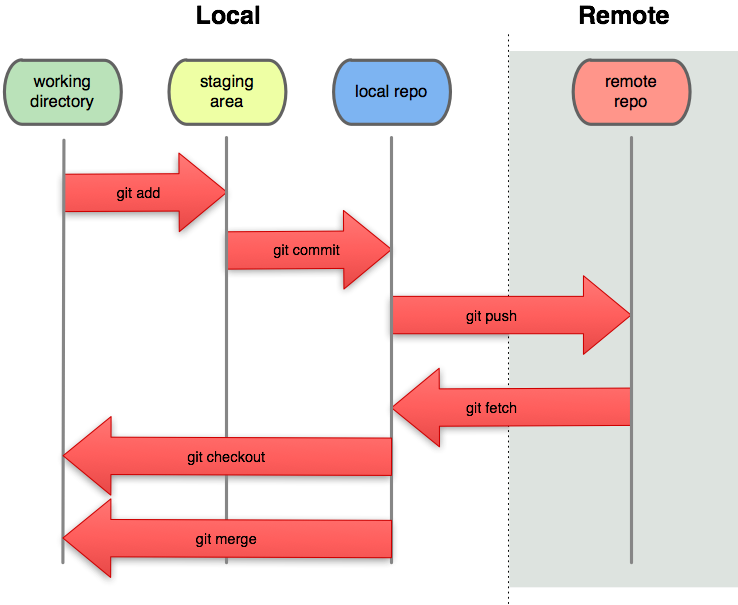
\includegraphics[width=0.75\textwidth]{git.png}
%\caption{Overview of git commands. Source: \url{https://kevintshoemaker.github.io/StatsChats/GIT_tutorial.html}}
%\label{fig:git}
%\end{figure}




\section{Where to find more information}
For a \emph{high-level overview} of Paparazzi and descriptions of file types such as the \emph{flight plan xml} or \emph{module xml}'s, refer to the Paparazzi wiki at \url{https://wiki.paparazziuav.org}.

For more in-depth descriptions of \emph{existing modules} and their defines, check out the auto-generated documentation at \url{http://docs.paparazziuav.org/latest/}. The content of these pages is generated directly from the module .xml files, which can be found in the \texttt{paparazzi/conf/modules} directory.

If you are experiencing \emph{issues with Paparazzi that are not caused by your own code}, check out the issue pages on Github (\url{https://github.com/paparazzi/paparazzi/issues}, \url{https://github.com/tudelft/paparazzi/issues}) to see if someone else is running into the same problem and if there is a temporary solution or fix.
\textbf{If you want to create a new issue, please do so on the tudelft fork of Paparazzi} (\url{https://github.com/tudelft/paparazzi/issues}).

If you really want to know \emph{what goes on inside the autopilot}, you can't get more detailed information than the source code itself! All of the autopilot code can be found in the \texttt{paparazzi/sw/airborne/} directory. The following files and directories are most relevant for the course:
\begin{itemize}
\item \texttt{paparazzi/sw/airborne/}
\begin{itemize}
\item \texttt{firmwares/rotorcraft/} - \emph{This folder contains the autopilot code that is shared between all types of rotorcraft. This includes guidance and stabilization code.}
\begin{itemize}
\item \texttt{guidance/} - \emph{Here you can find the guidance controllers. The controller is split into a horizontal part (guidance\_h) and a vertical part (guidance\_v).}
\item \texttt{stabilization/} - \emph{This folder contains the stabilization controllers. The example airframe uses the stabilization\_indi\_simple controller.}
\item \texttt{autopilot\_guided.h} - \emph{This header allows you to set position and velocity setpoints while flying in GUIDED mode.} \textbf{TODO should probably be guidance\_h.h!}
\item \texttt{main.c} - \emph{If you were wondering if Paparazzi also has a `main' function, here it is. After initializing the autopilot, the main function will loop indefinitely while performing its periodic tasks.}
\item \texttt{navigation.h} - \emph{These functions are commonly called from the flight plan.}
\end{itemize}
\item \texttt{math/} - \emph{Here you can find math functions for matrix and vector operations in Paparazzi. These are documented in paparazzi/doc/pprz\_algebra/headfile.pdf. Pprz\_algebra\_float.h might be a good starting point for general-purpose floating point calculations.}
\item \texttt{modules/} - \emph{Here you find the code for modules that other people have written. Be sure to check out how these modules are written if you're looking for inspiration.}
\begin{itemize}
\item \texttt{computer\_vision/} - \emph{This folder contains the computer vision code. Use the functions in cv.h to register your video callback.}
\end{itemize}
\item \texttt{state.h} - \emph{Use this header to read the current state of the UAV. Use the stateGet... functions.}
\end{itemize}
\end{itemize}

The autopilot code is spread over a large number of files. Use Eclipse to navigate these files effectively. Hovering over a variable or function will show its definition and hopefully some descriptive comments. Ctrl+clicking on a variable will take you to its definition or declaration. Ctrl+clicking will also allow you to quickly open header files, then use Ctrl+Tab to open the corresponding source file.
If `Mark Occurrences' (Shift+Alt+O) is turned on, placing your text cursor on the variable name will highlight all occurrences in the file you have opened.
To see how a variable is used across files, right click it and choose `References $\rightarrow$ Project'.
Finally, `Search' (Ctrl+H) allows you to search arbitrary text in all files. Set `Scope' to `Selected resources' to limit your search to the folder you have selected in the Project Explorer.

If your question is not answered by these resources or if you don't know where to look, feel free to ask the TA's for advice.

\end{document}
